\documentclass{article}

\usepackage[margin=1in]{geometry}
\usepackage{amsmath,amsthm,amssymb}
\usepackage{bbm,enumerate,mathtools,mathrsfs}
\usepackage[hidelinks]{hyperref}
\usepackage{tikz}
\usetikzlibrary{matrix, arrows}

\newenvironment{problem}[2][Problem]{\begin{trivlist}
\item[\hskip \labelsep {\bfseries #1}\hskip \labelsep {\bfseries #2.}]}{\end{trivlist}}
\newenvironment{solution}[1][Solution.]{\begin{trivlist}
\item[\hskip \labelsep {\bfseries #1}]}{\end{trivlist}}
\newenvironment{problempart}[1]{\begin{trivlist}\item[\textbf{Part #1.}]}{\end{trivlist}}

\newenvironment{definition}[1][Definition.]{
  \begin{trivlist} \item[\hskip \labelsep {\bfseries #1}]
}{\end{trivlist}}

\newenvironment{example}[1][Example.]{
  \begin{trivlist} \item[\hskip \labelsep {\bfseries #1}]
}{\end{trivlist}}

\newenvironment{note}[1][Note.]{
  \begin{trivlist} \item[\hskip \labelsep {\bfseries #1}]
}{\end{trivlist}}

\newenvironment{theorem}[1][Theorem.]{
  \begin{trivlist} \item[\hskip \labelsep {\bfseries #1}]
}{\end{trivlist}}

\newenvironment{exercise}[1][Exercise.]{
  \begin{trivlist} \item[\hskip \labelsep {\bfseries #1}]
}{\end{trivlist}}

\newcommand{\set}[1]{\{ #1 \}}
\newcommand{\ang}[1]{\langle #1 \rangle}
\newcommand{\paren}[1]{\left( #1 \right)}
\newcommand{\fn}[3]{#1 \colon #2 \rightarrow #3}
\newcommand{\wt}{\operatorname{wt}}
\newcommand{\id}{\operatorname{id}}

\begin{document}

\title{Math 533: Homework 5}
\author{Peter Kagey}
\date{Friday, March 8, 2019}

\maketitle

% -----------------------------------------------------
% First problem
% -----------------------------------------------------
\begin{problem}{1}
\end{problem}

\begin{proof} ~
  \begin{enumerate}[(a)]
    \item Given some filling, remove as many primes as possible, and call this
    the minimal filling. This can be
    done unambiguously, because there is at most one $i'$ per row.
    Now there are $2^\ell(\gamma)$ ways of priming elements. In particular, each
    row has at least one ``primeable'' element, all independent.
    Since there are $\ell(\gamma)$ rows, this means that for each minimal
    filling, there are a multiple of $2^\ell(\gamma)$ fillings with the same
    weight.
    \item When $\gamma$ is a strict partition, the shifted tableau can be
    partitioned into a ``staircase'' and a Young tableau. \[
      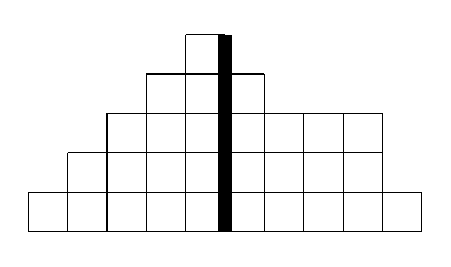
\begin{tikzpicture}[scale=0.5]
        \draw (0,0) grid (10,1);
        \draw (1,1) grid (9,2);
        \draw (2,2) grid (9,3);
        \draw (3,3) grid (6,4);
        \draw (4,4) grid (5,5);
        \draw[line width=5] (5,0)--(5,5);
      \end{tikzpicture}
    \]
    Now consider a modified Bender-Knuth involution: hold constant any pairs (ignoring primes) \[
    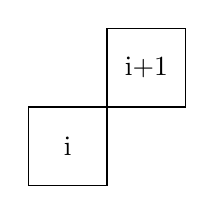
\begin{tikzpicture}[scale=0.5]
      \draw (0,0) rectangle (2,2);
      \draw (2,2) rectangle (4,4);
      \node at (1,1) {i};
      \node at (3,3) {i+1};
    \end{tikzpicture}
    \] Now all that remains is horizontal strips of the form \[
      \underbrace{i, i, \hdots, i}_a, \underbrace{i+1, i+1, \hdots, i+1}_b
    \] map these strips to \[
      \underbrace{i, i, \hdots, i}_b, \underbrace{i+1, i+1, \hdots, i+1}_a
    \] adding primes when vertical dominoes force it and removing primes when
    horizontal dominoes force it.
    \item From the previous homework, it is enough to show that
    $Q_\gamma(x_1,-x_1,x_3,x_4,\hdots) = Q_\gamma(x_3,x_4,\hdots)$
  \end{enumerate}
\end{proof}
\pagebreak
% -----------------------------------------------------
% Second problem
% -----------------------------------------------------
\begin{problem}{2}
\end{problem}

\begin{proof} ~
  \begin{enumerate}
    \item[(c)] For an involution, the inner structure is cycles of length one or
    two, which has exponential generating function $x+x^2/2$, and the outer
    structure puts such cycles together, so the appropriate generating function is $\exp(x + x^2/2)$.
  \end{enumerate}
\end{proof}
\pagebreak
% % -----------------------------------------------------
% % Third problem
% % -----------------------------------------------------
% \begin{problem}{3}
%   Pieri's rule states that \[
%     s_\lambda \cdot h_n = \sum_{\lambda^+ \supseteq \lambda} s_{\lambda^+}
%   \] where $\lambda^+ \setminus \lambda$ is a horizontal strip of length $n$.
%
%   % By modified RSK.
%   % We know that $h_\mu = \sum_{\lambda} K_{\lambda\mu}s_\lambda$ where
%   % $h_\mu$ is the homogenous symmetric function of shape $\mu$,
%   % $K_{\lambda\mu}$ is the Kostka number of shape $\lambda$ and weight $\mu$,
%   % and $s_\lambda$ is the Shur function of shape $\lambda$. Thus \begin{align*}
%   %   s_{\lambda/(1)}\cdot h_n
%   %   &= s_{\lambda/(1)} \cdot \sum_{\mu} K_{\mu(n)}s_\mu \\
%   %   &= \sum_{\mu} K_{\mu(n)}s_{\lambda/(1)} \cdot s_\mu \\
%   %   &= \sum_{\mu}\sum_{\nu} K_{\mu(n)}c^\lambda_{(1)\nu} s_\nu \cdot s_\mu \\
%   %   &= \sum_{\mu,\nu} K_{\mu(n)}\ang{s_{(1)}s_\nu, s_\lambda} s_\nu \cdot s_\mu
%   % \end{align*}
% \end{problem}
%
% \begin{proof}
% \end{proof}
% -----------------------------------------------------
% Fourth problem
% -----------------------------------------------------
\begin{problem}{4}
\end{problem}

\begin{proof} ~
  \begin{enumerate}[(a)]
    \item $a(n)$ is equivalent to a Catalan walk: insert $\set{1, 2, \hdots, 2n}$ in
    order, $i$ can only go in the second row if there are strictly more
    elements in the first row. This is equivalent to a walk that stays above
    the diagonal. (Placing a number in the first row is a step up, and
    placing a number in the second row is a step right.) Thus \[
      a(n) = \frac{1}{n+1}\binom{2n}{n}
    \]
    \item $b(n)$ the number of $n$-step walks that stay above the diagonal. This is
    because we can always add to the second row if strictly more
    letters (respectively vertical steps) have been added to the first row.
    This is given by \[
      b(n) = \binom{n}{\lfloor \frac n 2 \rfloor}.
    \]
    \item
    There is a bijection between pairs of standard Young Tableaux of shape
    $\lambda$ and standard young Tableaux of shape $(n, n)$. The idea is to
    ``flip'' the second standard Young Tableau, and reindex by mapping all
    entries to $k \mapsto 2n + 1 - k$. For example, \[
      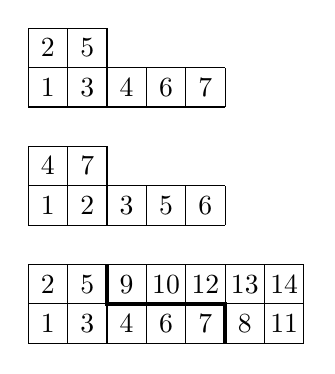
\begin{tikzpicture}[scale=0.5]
        \draw (0,0) grid (5,1);
        \draw (0,1) grid (2,2);

        \draw (0,3) grid (5,4);
        \draw (0,4) grid (2,5);

        \draw (0,-3) grid (7,-1);
        \draw[ultra thick] (2,-1)--(2,-2)--(5,-2)--(5,-3);
        \foreach \i/\x/\y in {
          1/3/0, 2/4/0, 3/3/1, 4/3/2, 5/4/1, 6/3/3, 7/3/4,
          1/0/0, 4/1/0, 2/0/1, 3/0/2, 7/1/1, 5/0/3, 6/0/4,
          1/-3/0, 2/-2/0, 3/-3/1, 4/-3/2, 5/-2/1, 6/-3/3, 7/-3/4,
          8/-3/5,11/-3/6, 9/-2/2,10/-2/3,12/-2/4,13/-2/5,14/-2/6
        } {
          \node at (\y + 0.5, \x + 0.5) {\i};
        }
      \end{tikzpicture}
    \] To recover the original pair: For the first tableau, take the sub-tableau that
    consists of entries up to $n$; for the second, take the complement, flip it, and
    re-apply the map. Therefore \[
      c(n) = a(n) = \frac{1}{n+1}\binom{2n}{n}.
    \]
    % This is the same as the number of pairs of shape
    % $(\lambda, \lambda^*)$, where as above, $\lambda$ is in bijection with
    % $n$-step walks that stay above the diagonal, and $\lambda^*$ gives an $n$-step
    % walk from the end of the $\lambda$-walk to $(n,n)$ such that the whole walk
    % stays above diagonal (due to the shape of $\lambda^*$.)
    % This is given by the Catalan numbers \[
    %   c(n) = \frac{1}{n+1}\binom{2n}{n}
    % \]
  \end{enumerate}
\end{proof}
\pagebreak
% -----------------------------------------------------
% Fifth problem
% -----------------------------------------------------
\begin{problem}{5}
  Prove that the crystal string operators \[
    S_i(b) = \begin{cases}
      f_i^{\wt(b)_i - \wt(b)_{i+1}}(b) & \wt(b)_i \geq \wt(b)_{i+1} \\
      e_i^{\wt(b)_{i+1} - \wt(b)_i}(b) & \text{otherwise}
    \end{cases}
  \] satisfy the relations
  \begin{enumerate}[(a)]
    \item $S_i^2(b) = b$,
    \item $S_i S_j(b) = S_j S_i(b)$ for $|i - j| > 1$, and
    \item $S_i S_{i+1} S_i(b) = S_{i+1} S_i S_{i+1}(b)$.
  \end{enumerate}
\end{problem}

\begin{proof} First, notice that by construction, $S_i(b)$ has the same weight
  as $b$, but with the values in the $i$ and $i+1$ positions switched. That is,
  if $\wt(b) = (w_1, w_2, \hdots, w_n)$ then
  $\wt(S_i(b)) = (w_1, w_2, \hdots, w_{i-1}, w_{i+1}, w_i, w_{i+2}, \hdots, w_n)$
  \begin{enumerate}[(a)]
    \item If $\wt(b)_i = \wt(b)_{i+1}$, then $S_i = \id$, so $S_i^2 = \id^2 = \id$.
    \\~\\
    If $\wt(b)_i - \wt(b)_{i+1} = k > 0$, then
    $S_i(b) = f_i^k(b)$, where $\wt(S_i(b))_{i+1} - \wt(S_i(b))_i = k$, so
    $S_i(S_i(b)) = e_i^k(f_i^k(b))$, then since function composition is
    commutative, and $f_i^k(b) \neq 0$, cancelling from the middle yields \[
      e_i^{k-1}\circ  e_i \circ  f_i \circ f_i^{k-1}
    \] where $e_i \circ f_i$ is the identity.
    \\~\\
    If $\wt(b)_{i+1} - \wt(b)_{i} = k > 0$, then
    $S_i(b) = e_i^k(b)$, where $\wt(S_i(b))_i - \wt(S_i(b))_{i+1} = k$, so
    $S_i(S_i(b)) = f_i^k(e_i^k(b))$, then since function composition is
    commutative, and $e_i^k(b) \neq 0$, cancelling from the middle yields \[
      f_i^{k-1}\circ f_i \circ  e_i \circ e_i^{k-1}
    \] where $f_i \circ e_i$ is the identity.
    \item I can't show that these functions commute, but I can show that they
    both result in elements with the same weight: the values in positions $i$ and
    then $i+1$ and then switching those in positions $j$ and $j+1$ is the same
    as doing it in the other order: \begin{alignat*}{2}
      (w_1, \hdots, w_i, w_{i+1}, w_{i+2}, \hdots, w_n)
      &\xmapsto{S_i}     &&\ (w_1, \hdots, w_{i+1}, w_i, \hdots, w_{j}, w_{j+1}, \hdots, w_n) \\
      &\xmapsto{S_j}     &&\ (w_1, \hdots, w_{i+1}, w_i, \hdots, w_{j+1}, w_{j}, \hdots, w_n) \\
      (w_1, \hdots, w_i, w_{i+1}, w_{i+2}, \hdots, w_n)
      &\xmapsto{S_{j}}   &&\ (w_1, \hdots, w_{i}, w_{i+1}, \hdots, w_{j+1}, w_{j}, \hdots, w_n) \\
      &\xmapsto{S_{i}}   &&\ (w_1, \hdots, w_{i+1}, w_i, \hdots, w_{j+1}, w_{j}, \hdots, w_n),
    \end{alignat*}
    So the commutator relation satisfies the weight condition.
    \item The same thing happens with the braid case \begin{alignat*}{2}
      (w_1, \hdots, w_i, w_{i+1}, w_{i+2}, \hdots, w_n)
      &\xmapsto{S_i}     &&\ (w_1, \hdots, w_{i+1}, w_i, w_{i+2}, \hdots, w_n) \\
      &\xmapsto{S_{i+1}} &&\ (w_1, \hdots, w_{i+1}, w_{i+2}, w_{i}, \hdots, w_n) \\
      &\xmapsto{S_{i}}   &&\ (w_1, \hdots, w_{i+2}, w_{i+1}, w_{i}, \hdots, w_n) \\
      (w_1, \hdots, w_i, w_{i+1}, w_{i+2}, \hdots, w_n)
      &\xmapsto{S_{i+1}} &&\ (w_1, \hdots, w_{i}, w_{i+2}, w_{i+1}, \hdots, w_n) \\
      &\xmapsto{S_{i}}   &&\ (w_1, \hdots, w_{i+2}, w_{i}, w_{i+1}, \hdots, w_n) \\
      &\xmapsto{S_{i+1}} &&\ (w_1, \hdots, w_{i+2}, w_{i+1}, w_{i}, \hdots, w_n),
    \end{alignat*}
    that is, the braids satisfy the weight condition.
  \end{enumerate}
\end{proof}
\end{document}
